\subsection{Extracting DOM-Related Characteristics} \label{Sec:extractDomRelatedInfo}
The DOM connects a test case to the web application's code. Therefore, we first need to analyze the DOM-based test suite and extract the following pieces of information: (1) DOM-related operations of the existing test suite that may have tight connection with the \javascript code, and (2) frequently accessed DOM properties, which are potentially influential in improving the fault finding capability of the test suite, but are left unchecked in the manually-written test suite.

\headbf{DOM-Related Operations}
Any written test case needs to check the correctness of the application's behaviour. In a DOM-based test case, the expected behaviour is checked through DOM-based assertions. A
DOM-based assertion is defined as $<domProps,expVal>$, where $domProps$ consists of one or more DOM element features (e.g. attribute, and/or textual value), and $expVal$ is the correct value expected by the assertion. In the rest of the paper, we call the DOM element feature as a DOM property. 
DOM-based assertions play a significant role in our approach as they guide us towards important portions of the underlying \javascript code that need to be checked in unit-level assertions.

\begin{figure}[!t]
  \centering
  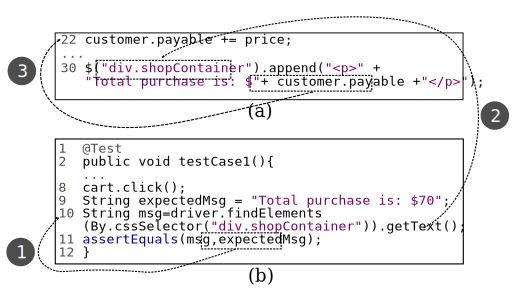
\includegraphics[width=1\hsize]{fig/intraDOMDep}
   \vspace{-0.3in} 
  \mycaption{Finding (1) intra DOM assertion dependency within the test case (b), (2) inter DOM assertion dependency between (b) DOM-based assertion and (a) the \javascript code, and (3) the initial point of contact between (b) DOM-based assertion and (a) the \javascript code.}
  \label{Fig:assertionToCode}
  \vspace{-0.2in} 
\end{figure}
For each DOM-based assertion we find \emph{intra DOM assertion dependency} within the test case.
\begin{mydef}[Intra DOM Assertion Dependency]
\label{def:intraDOMDep}  

An intra DOM assertion dependency is defined as a three tuple of $<assert, domElems, domProps>$, where $assert$ is the intended DOM-based assertion, $domElems$ is the accessed DOM elements in the test case pertaining to the assertion, and $domProps$ is the accessed DOM properties within the assertion.
\end{mydef}
\textsc{GetDomAcc} in line 10 of \algref{algorithm} retrieves DOM dependencies of the assertion in the test case.
%, we instrument the test case by wrapping around method calls that accesses DOM elements.
Going back to our example in \figref{assertionToCode}(b), tracking the assertion in line 11 shows that it has a DOM dependency to a \code{div} element with class \code{shopContainer}, which is accessed in line 10. The intra DOM assertion dependency of the example further shows that the \code{text} value of the DOM element is compared with the \code{expectedMsg} in line 11.    

We further need to correlate the inferred intra DOM assertion dependency with the application's code.
We call the correlation between the DOM-based assertion and the application's code as \emph{inter DOM assertion dependency}.

\begin{mydef}[Inter DOM Assertion Dependency]
\label{def:interDOMDep}  
An inter DOM assertion dependency is defined as
$<assert, initPoint>$, where $assert$ is the intended DOM-based assertion, and $initPoint$ is the initial line of code in the application that is responsible for mutating the property of a DOM element extracted from the intra DOM assertion dependency.
\end{mydef}
In order to find the initial point of contact between the application's code and a mutated DOM property in the DOM-based test case, we track evolution of the accessed DOM elements (\textsc{GetDomMuts} in line 13 of the algorithm) as well as invoked event handlers as the test case runs. 
We consider DOM mutation as a DOM-tree structural change (e.g.; additions and removals of child nodes), as well as DOM write operations such as changes to attributes and/or updates to child text nodes. For instance, running the sample test case in \figref{example}(b) results in mutating (1) the textual value of \code{div} element with class \code{shopContainer}, and (2) the \code{class} attribute of DOM element with ID \code{couponButt}.

In \secref{domToCode}, we explain inferring the initial point of contact between the source code and a mutated DOM element in a DOM-based test suite in details.  
%We call the correlation between the DOM-based assertion and the \javascript code of the application as \emph{inter DOM assertion correlation}. This correlation is defined as $<AccDOMDep, InitCode>$, where $InitCode$ is the initial point of contact in the application's code segment, that is responsible for mutating the previously extracted DOM elements from the test suite ($AccDOMDep$).  
%We make use of \code{document.onload} event to log the initial DOM state. 
%An observer module is then used to monitor mutations on the DOM during the test case execution. 
%In addition to DOM changes, we also keep track of \javascript events as well as invoked event handlers. This information is later used to find the initial point of contact between a DOM mutation and the executed code segments.
%For instance, running the sample test case in \figref{example}(b) results in mutating (1) the textual value of \code{div} element with class \code{shopContainer}, and (2) the \code{class} attribute of DOM element with ID \code{couponButt}.
\headbf{Frequently Accessed DOM Properties}
In addition to DOM-based assertions, we further consider DOM element properties that are frequently accessed within the application as the test case runs (lines 1 to 7 of \algref{algorithm}). 
\textsc{Acc} in line 6 of the algorithm computes the access frequency of a DOM property, $freqAccdDOM$ in line 7 contains the inferred candidate DOM properties, and \textsc{GetDomMuts} in line 19 records DOM mutations occur
on candidate DOM properties.

The intuition is that frequent use of a given DOM property can point to the extent of application's behaviour dependency on the DOM property. Thus, if changes happen to a property through the \javascript code, it is important to assert the correctness of mutations on the property. We define the access frequency of a DOM element property as the number of times that the element's property has been read during the execution of a test case. DOM properties include attributes as well as textual value of the elements.
In order to record DOM property accesses within the application, we rewrite native function calls used by programmers to access DOM element such as \code{getElementById}, \code{getElementsByClassName}, and/or \code{getElementsByTagName}. The returned object from these functions is later used to access attributes or textual values of the element. Thus, we apply a forward slice on the returned object to find instances of element's property access in the code.
For example in function \code{addToCart} of \figref{example}(a), DOM element with ID \code{couponButt} is assigned to \code{coupElem} variable. The assigned variable is later used to access the \code{class} attribute as well as the \code{value}
of the DOM element in lines 16, 18, and 19.

Let $Acc(prop_{el})$ be the access frequency computed for property $prop$ of DOM element $el$, then:
 
$Acc(prop_{el})=\frac{Read(prop_{el})}{\sum _{e=1}^{n} Read(domElem_e)}$, where $Read(domElem_{e})$ is the number of times that DOM element $domElem$ is read, given that the total number of DOM elements during the execution of a test case is $n$.
Note that reading a DOM element refers to accessing the element to read the corresponding property. In \figref{example}(a), the \code{class} attribute of DOM element \code{couponButt} is read in lines 16 and 27, and thus the access frequency
computed for the \code{class} attribute of the element is equal to $\frac{2}{3}$.

We choose element's property with access frequencies above a threshold $\alpha$ as potential candidates, which are later used for the purpose of unit-level assertion generation. We automatically compute this threshold for each test case as: 

$\alpha=\frac{1}{ReadProperties(T)}$, where $ReadProperties(T)$ is the total number of properties which have been read during the execution of test suite $T$.

Going back to our running example and the sample DOM-based test case in \figref{example}, \code{class} attribute of the \code{couponButt} is selected as a potential candidate since its access frequency ($\frac{2}{3}$) is greater than the computed threshold, which is equal to $\frac{1}{2}$ in this example.        
%application instrumentaion native event wrapping    
